\chapter{Results}
\label{chapter:results}
In this chapter we present quadrangulations of various input triangle-meshes, produced using a simple design tool we've built to demonstrate our method. Each figure is order from left to right, and top to bottom, and include a screenshot of the system's initial state upon loading an input triangle-mesh model, and a few screen captures from different point-of-views, of the final quadrangulation result. Singular-points are highlighted in red. Each input triangle-mesh was simplified to include 600 faces.
\newpage
\section{Bunny Model}
\begin{figure}[ht]
\centering
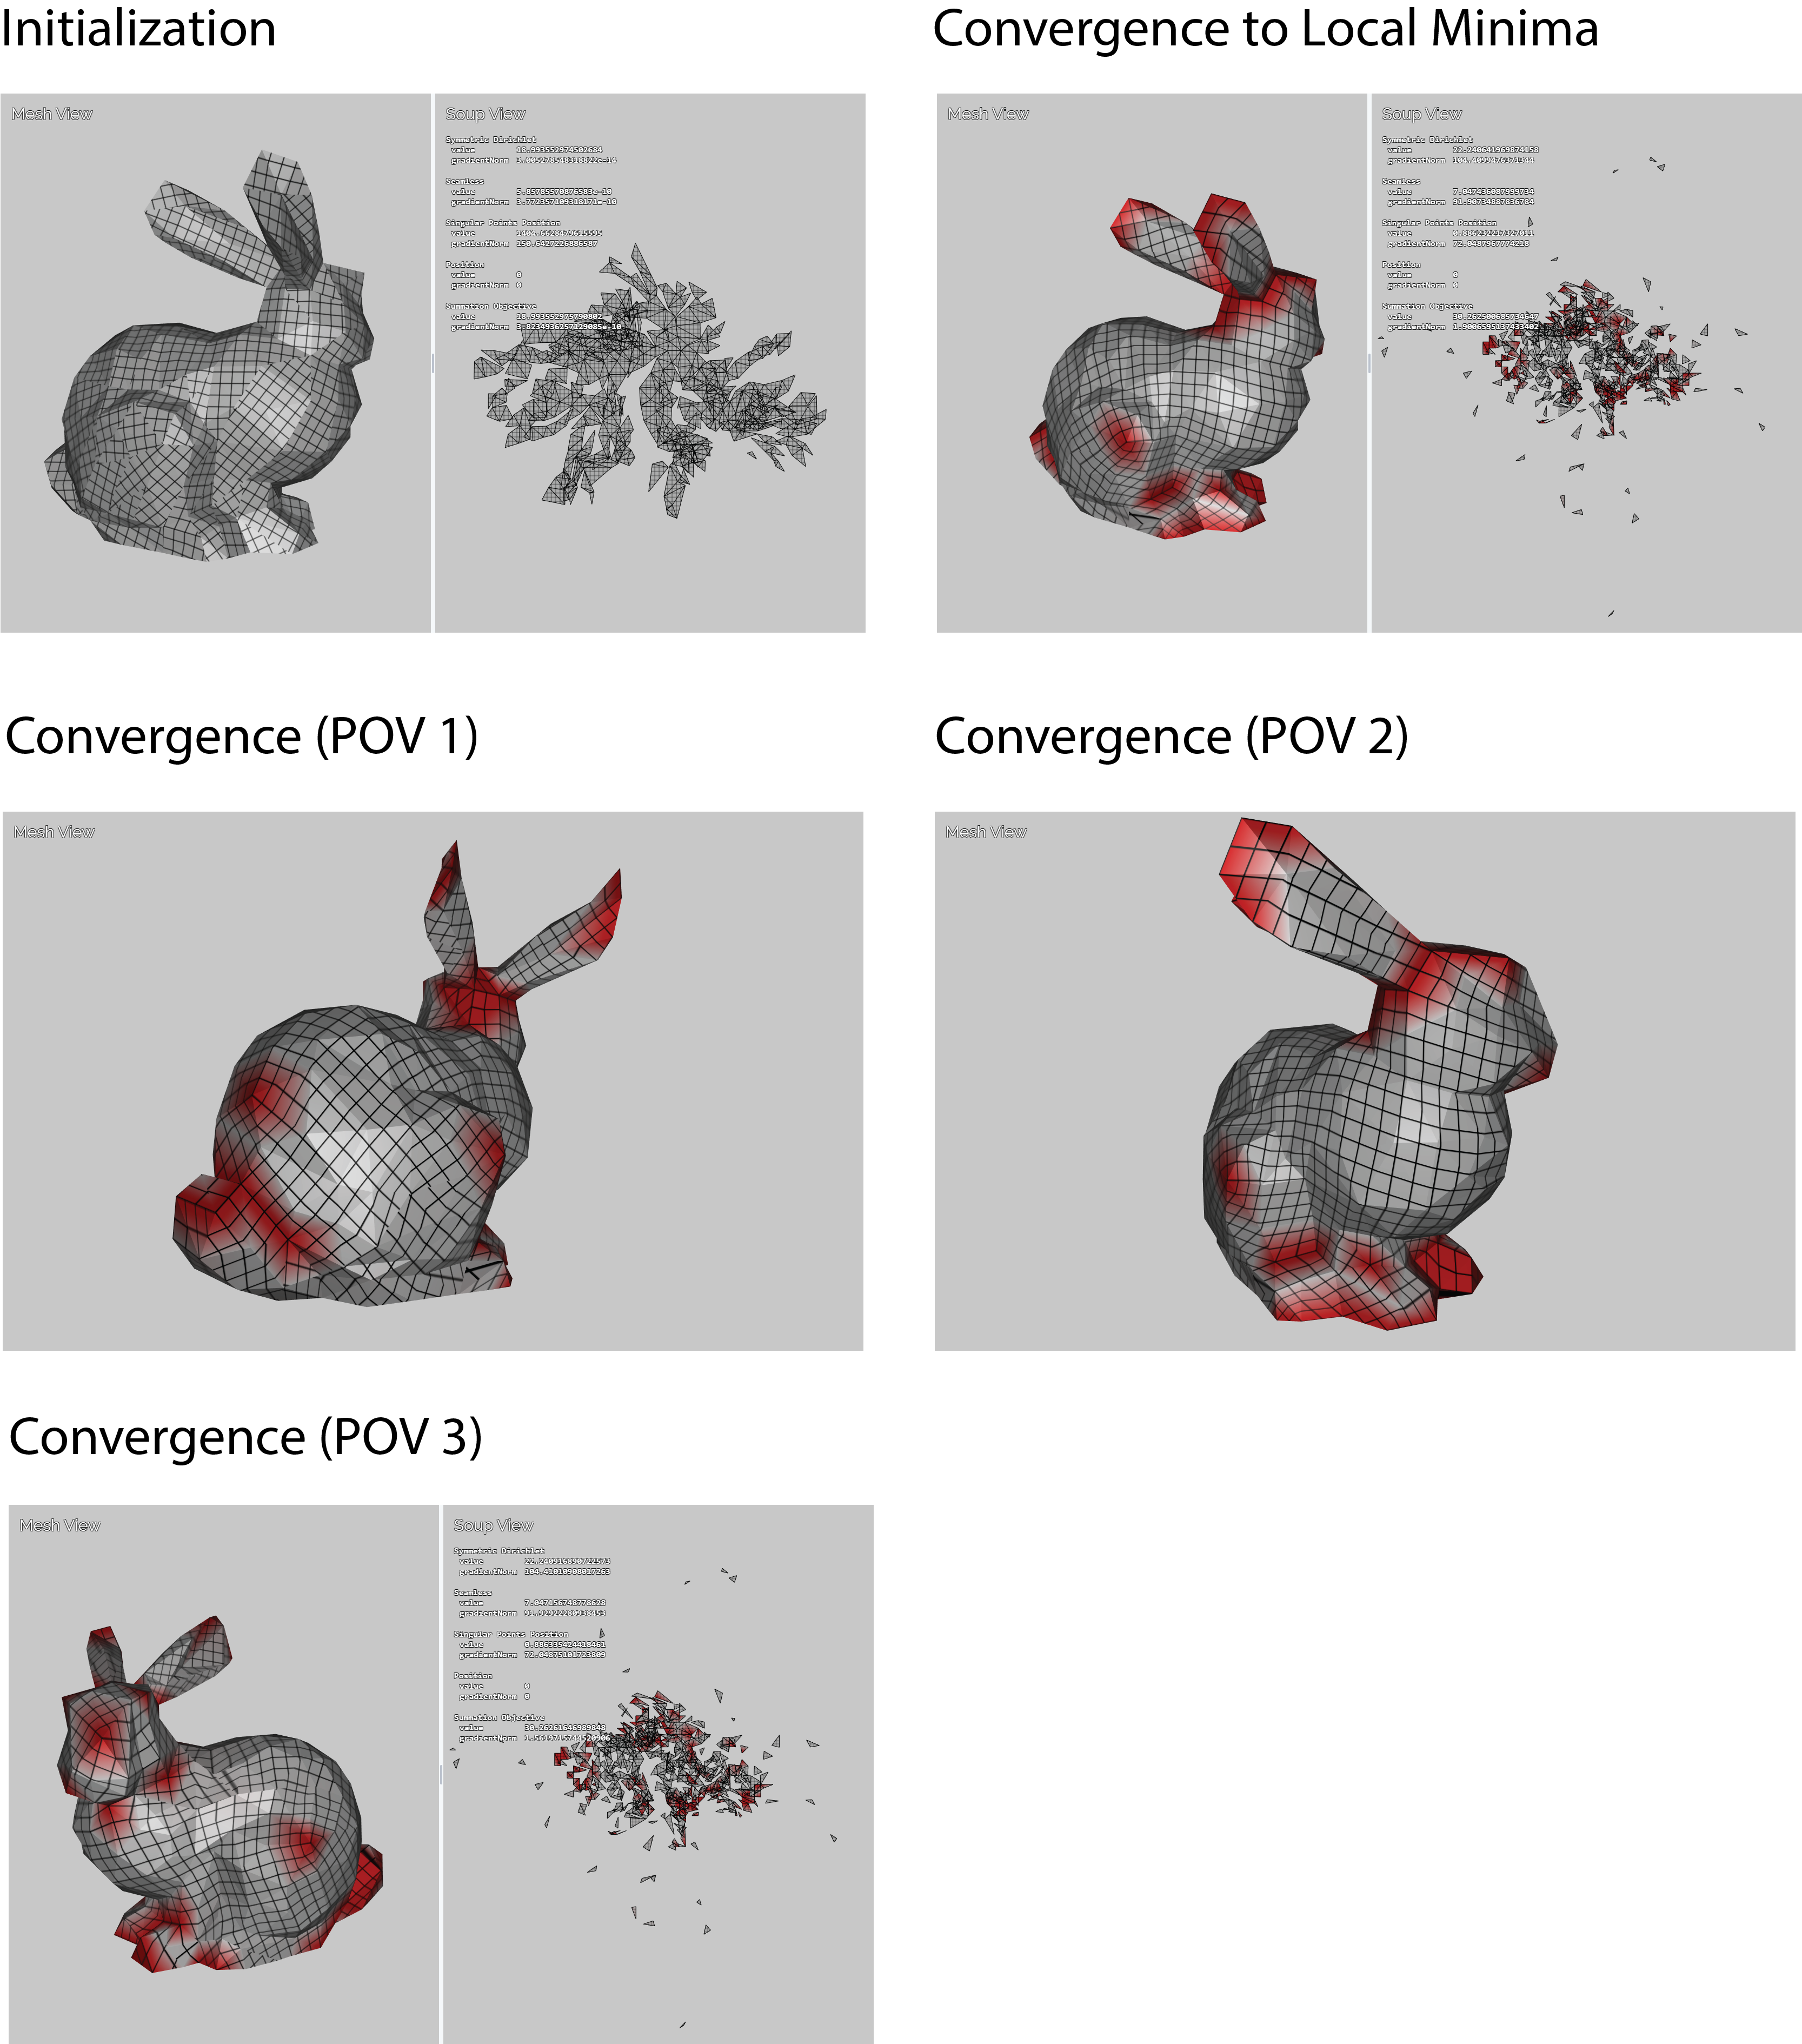
\includegraphics[width=14cm]{figures/results/bunny.png}
\caption[Bunny Model]{}
\end{figure}
\newpage
\section{Teddy Bear Model}
\begin{figure}[ht]
\centering
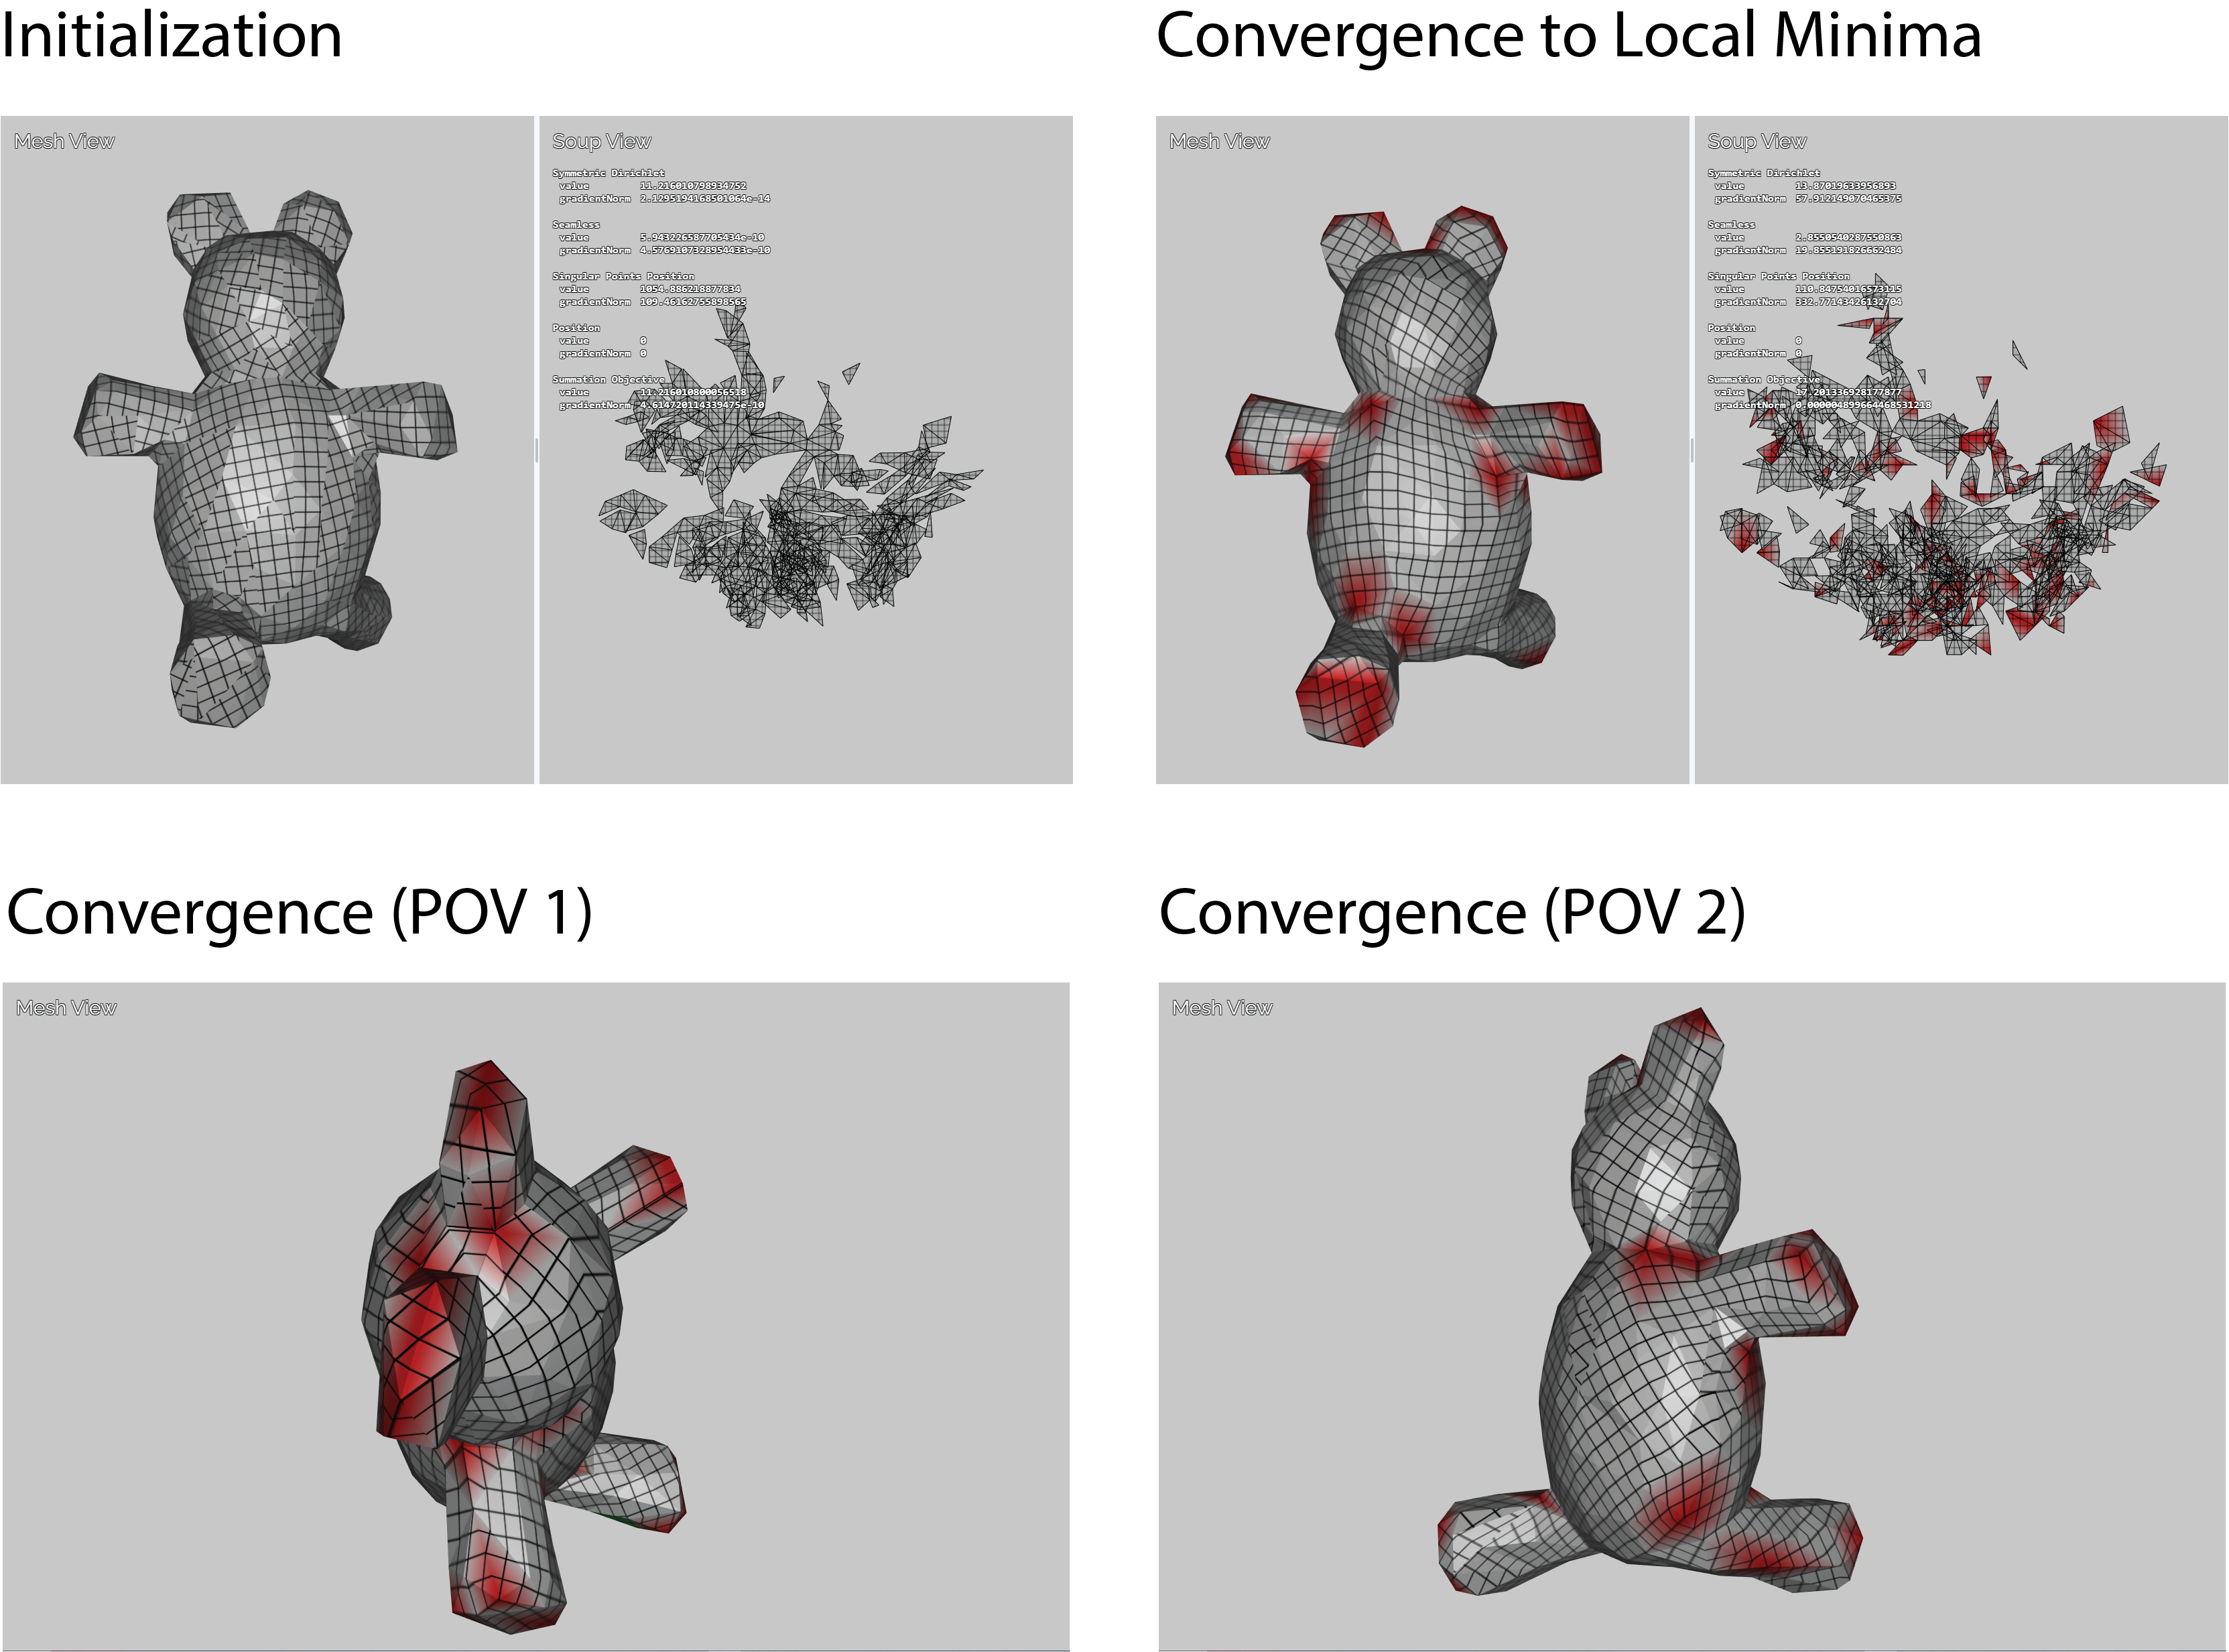
\includegraphics[width=14cm]{figures/results/teddy.png}
\caption[Teddy Bear Model]{}
\end{figure}
\newpage
\section{Kitten Model}
\begin{figure}[ht]
\centering
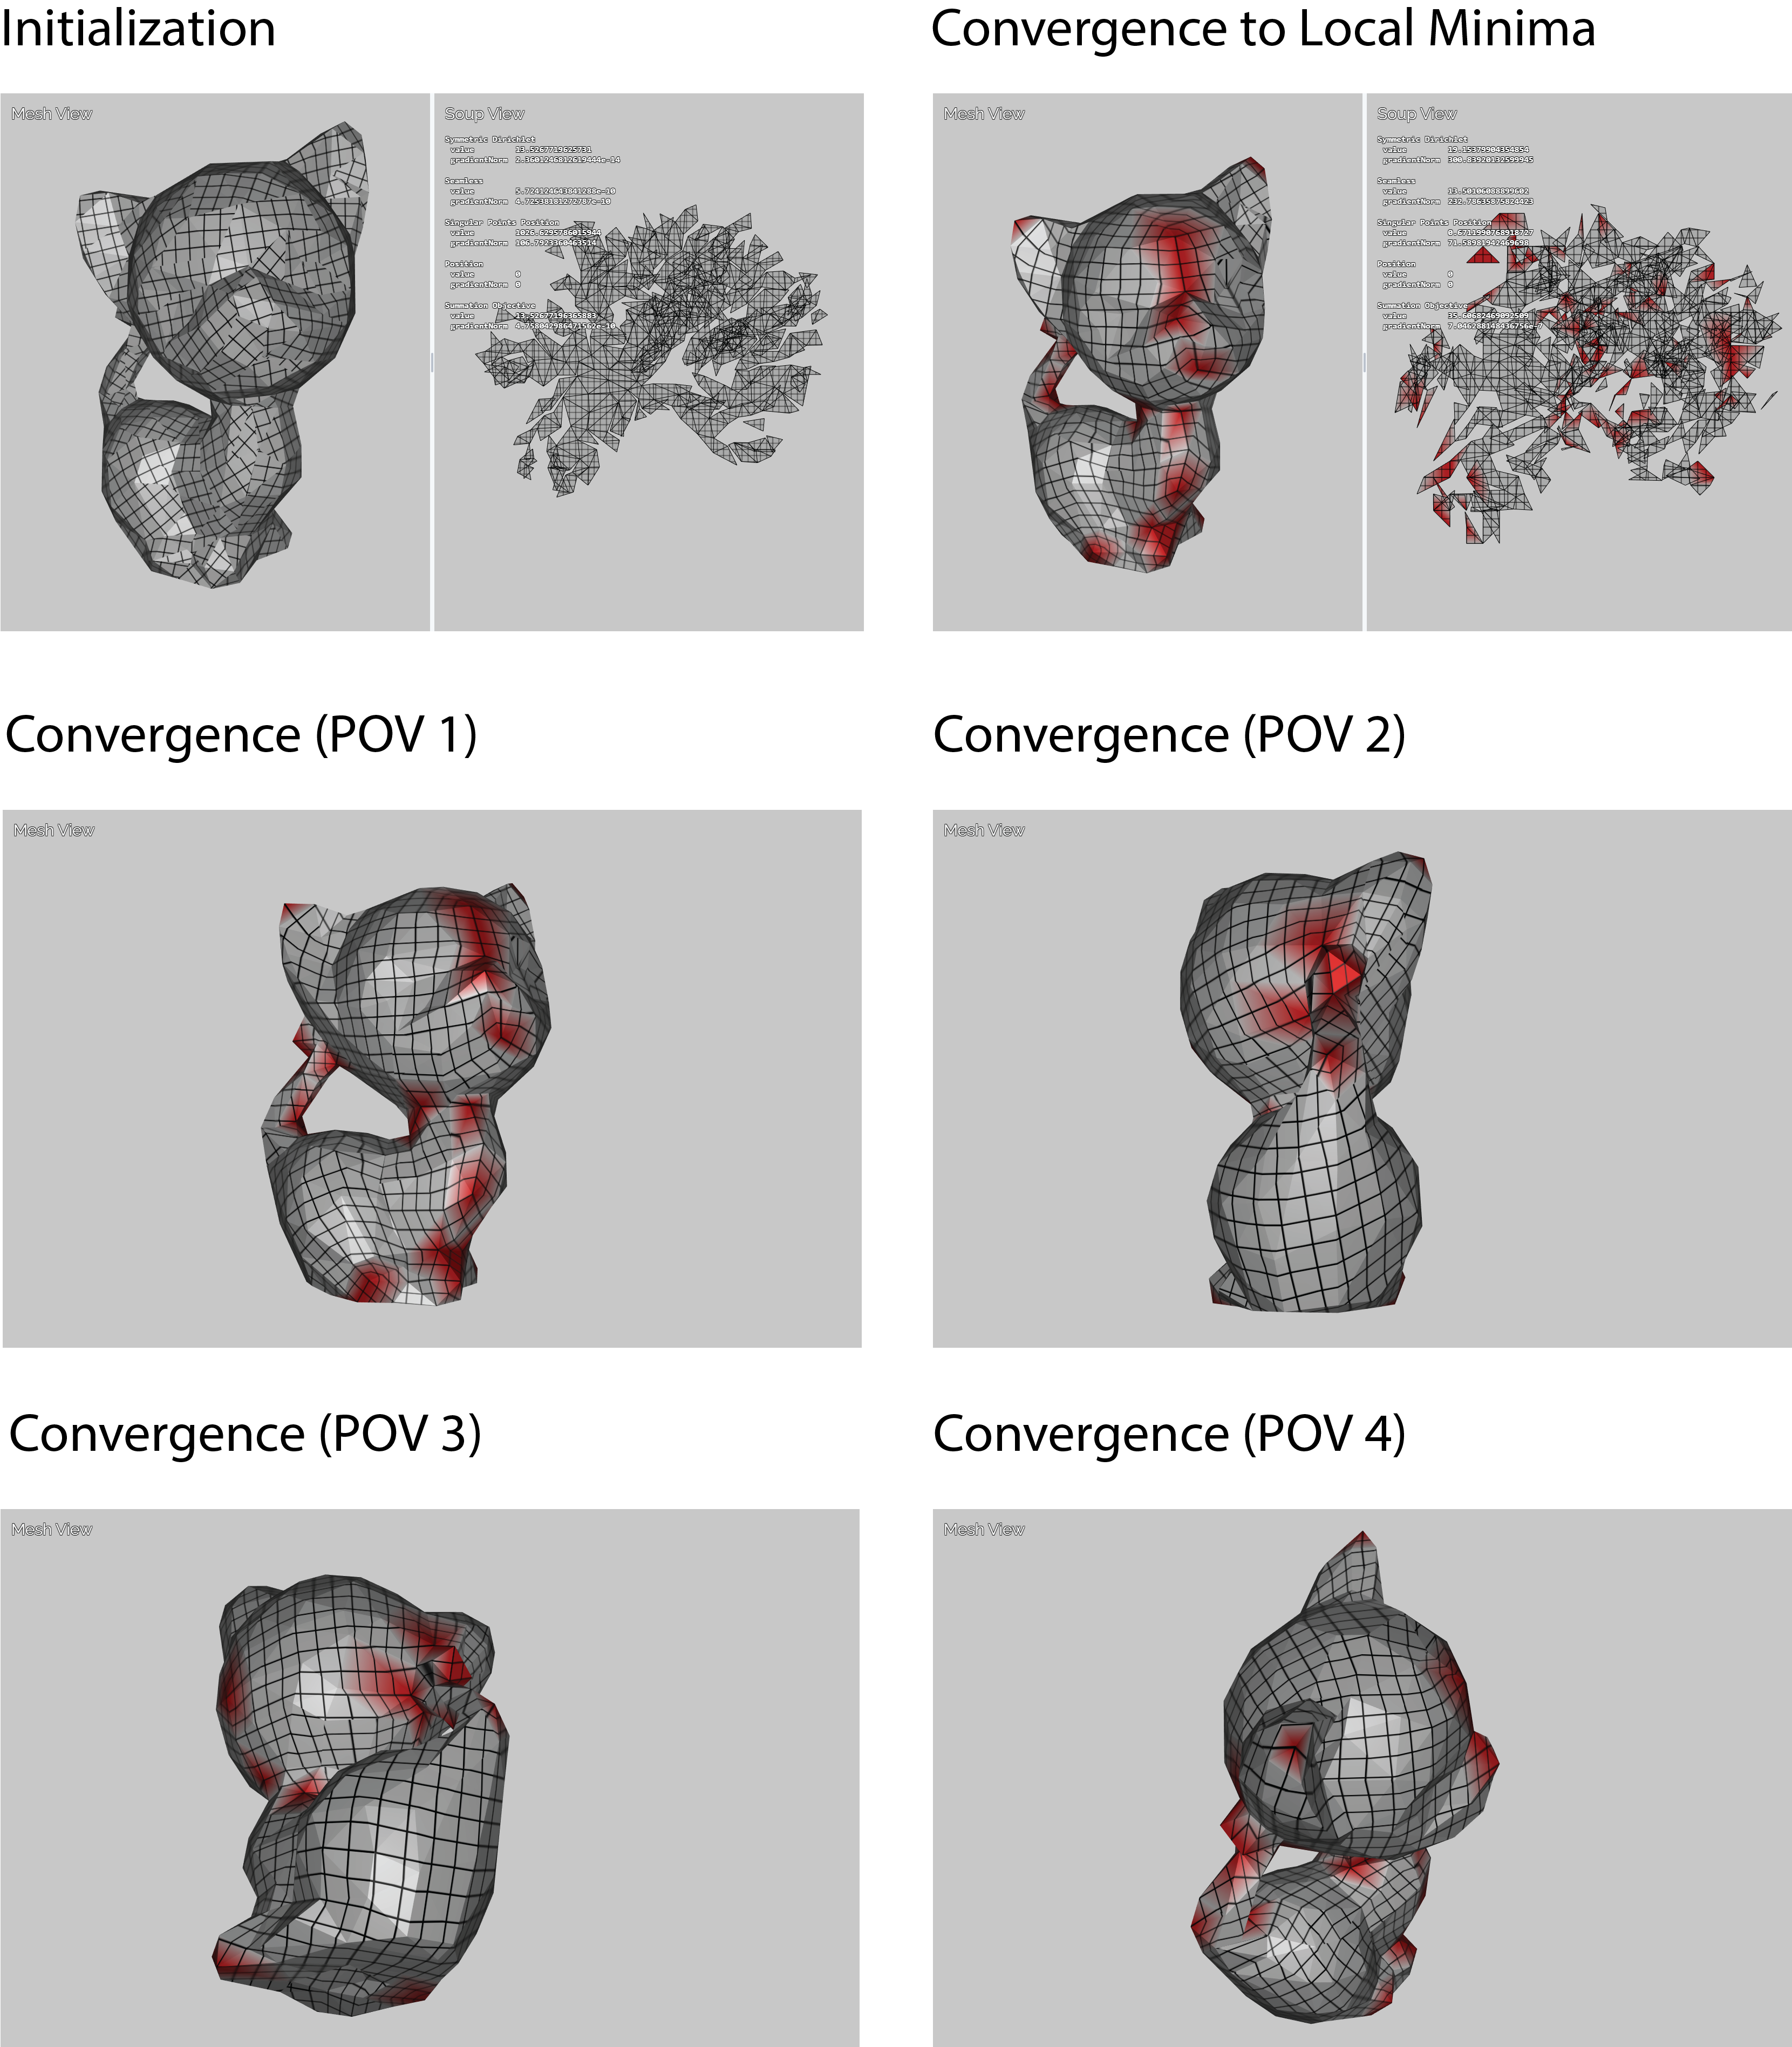
\includegraphics[width=14cm]{figures/results/kitten.png}
\caption[Kitten Model]{}
\end{figure}
\newpage
\section{Octopus Model}
\begin{figure}[ht]
\centering
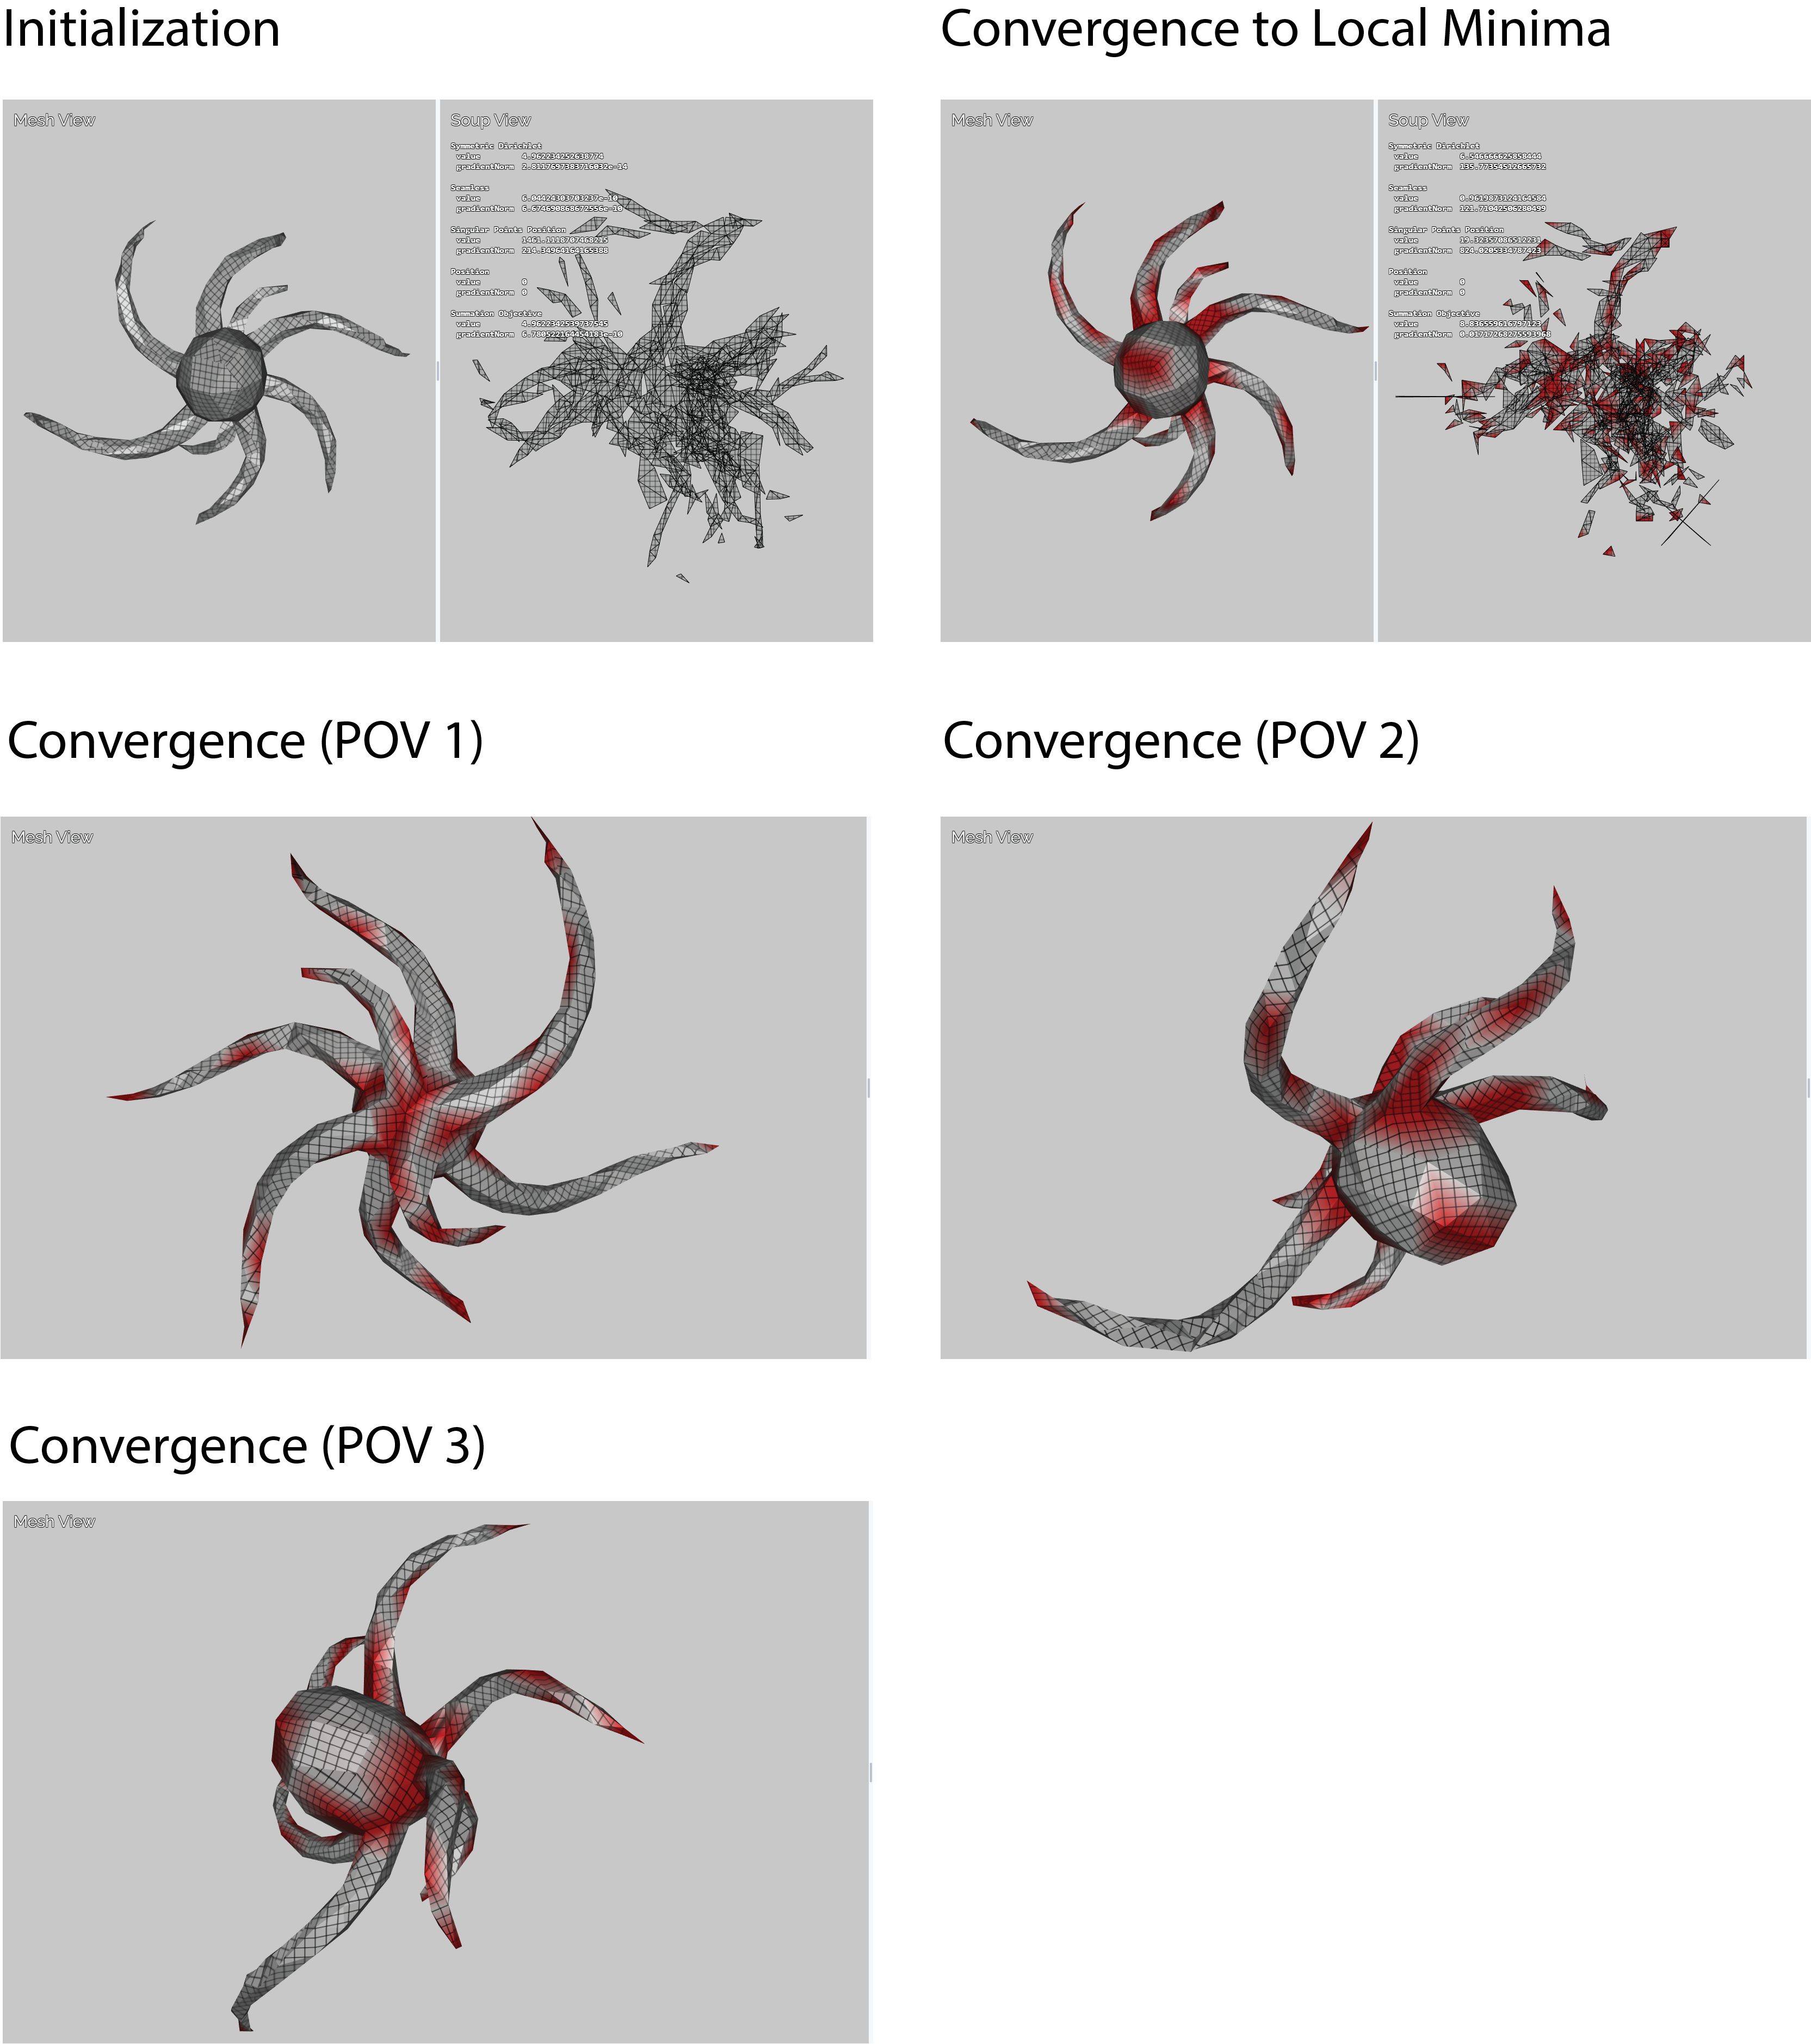
\includegraphics[width=14cm]{figures/results/octopus.png}
\caption[Octopus Model]{}
\end{figure}
\newpage
\section{Venus Model}
\begin{figure}[ht]
\centering
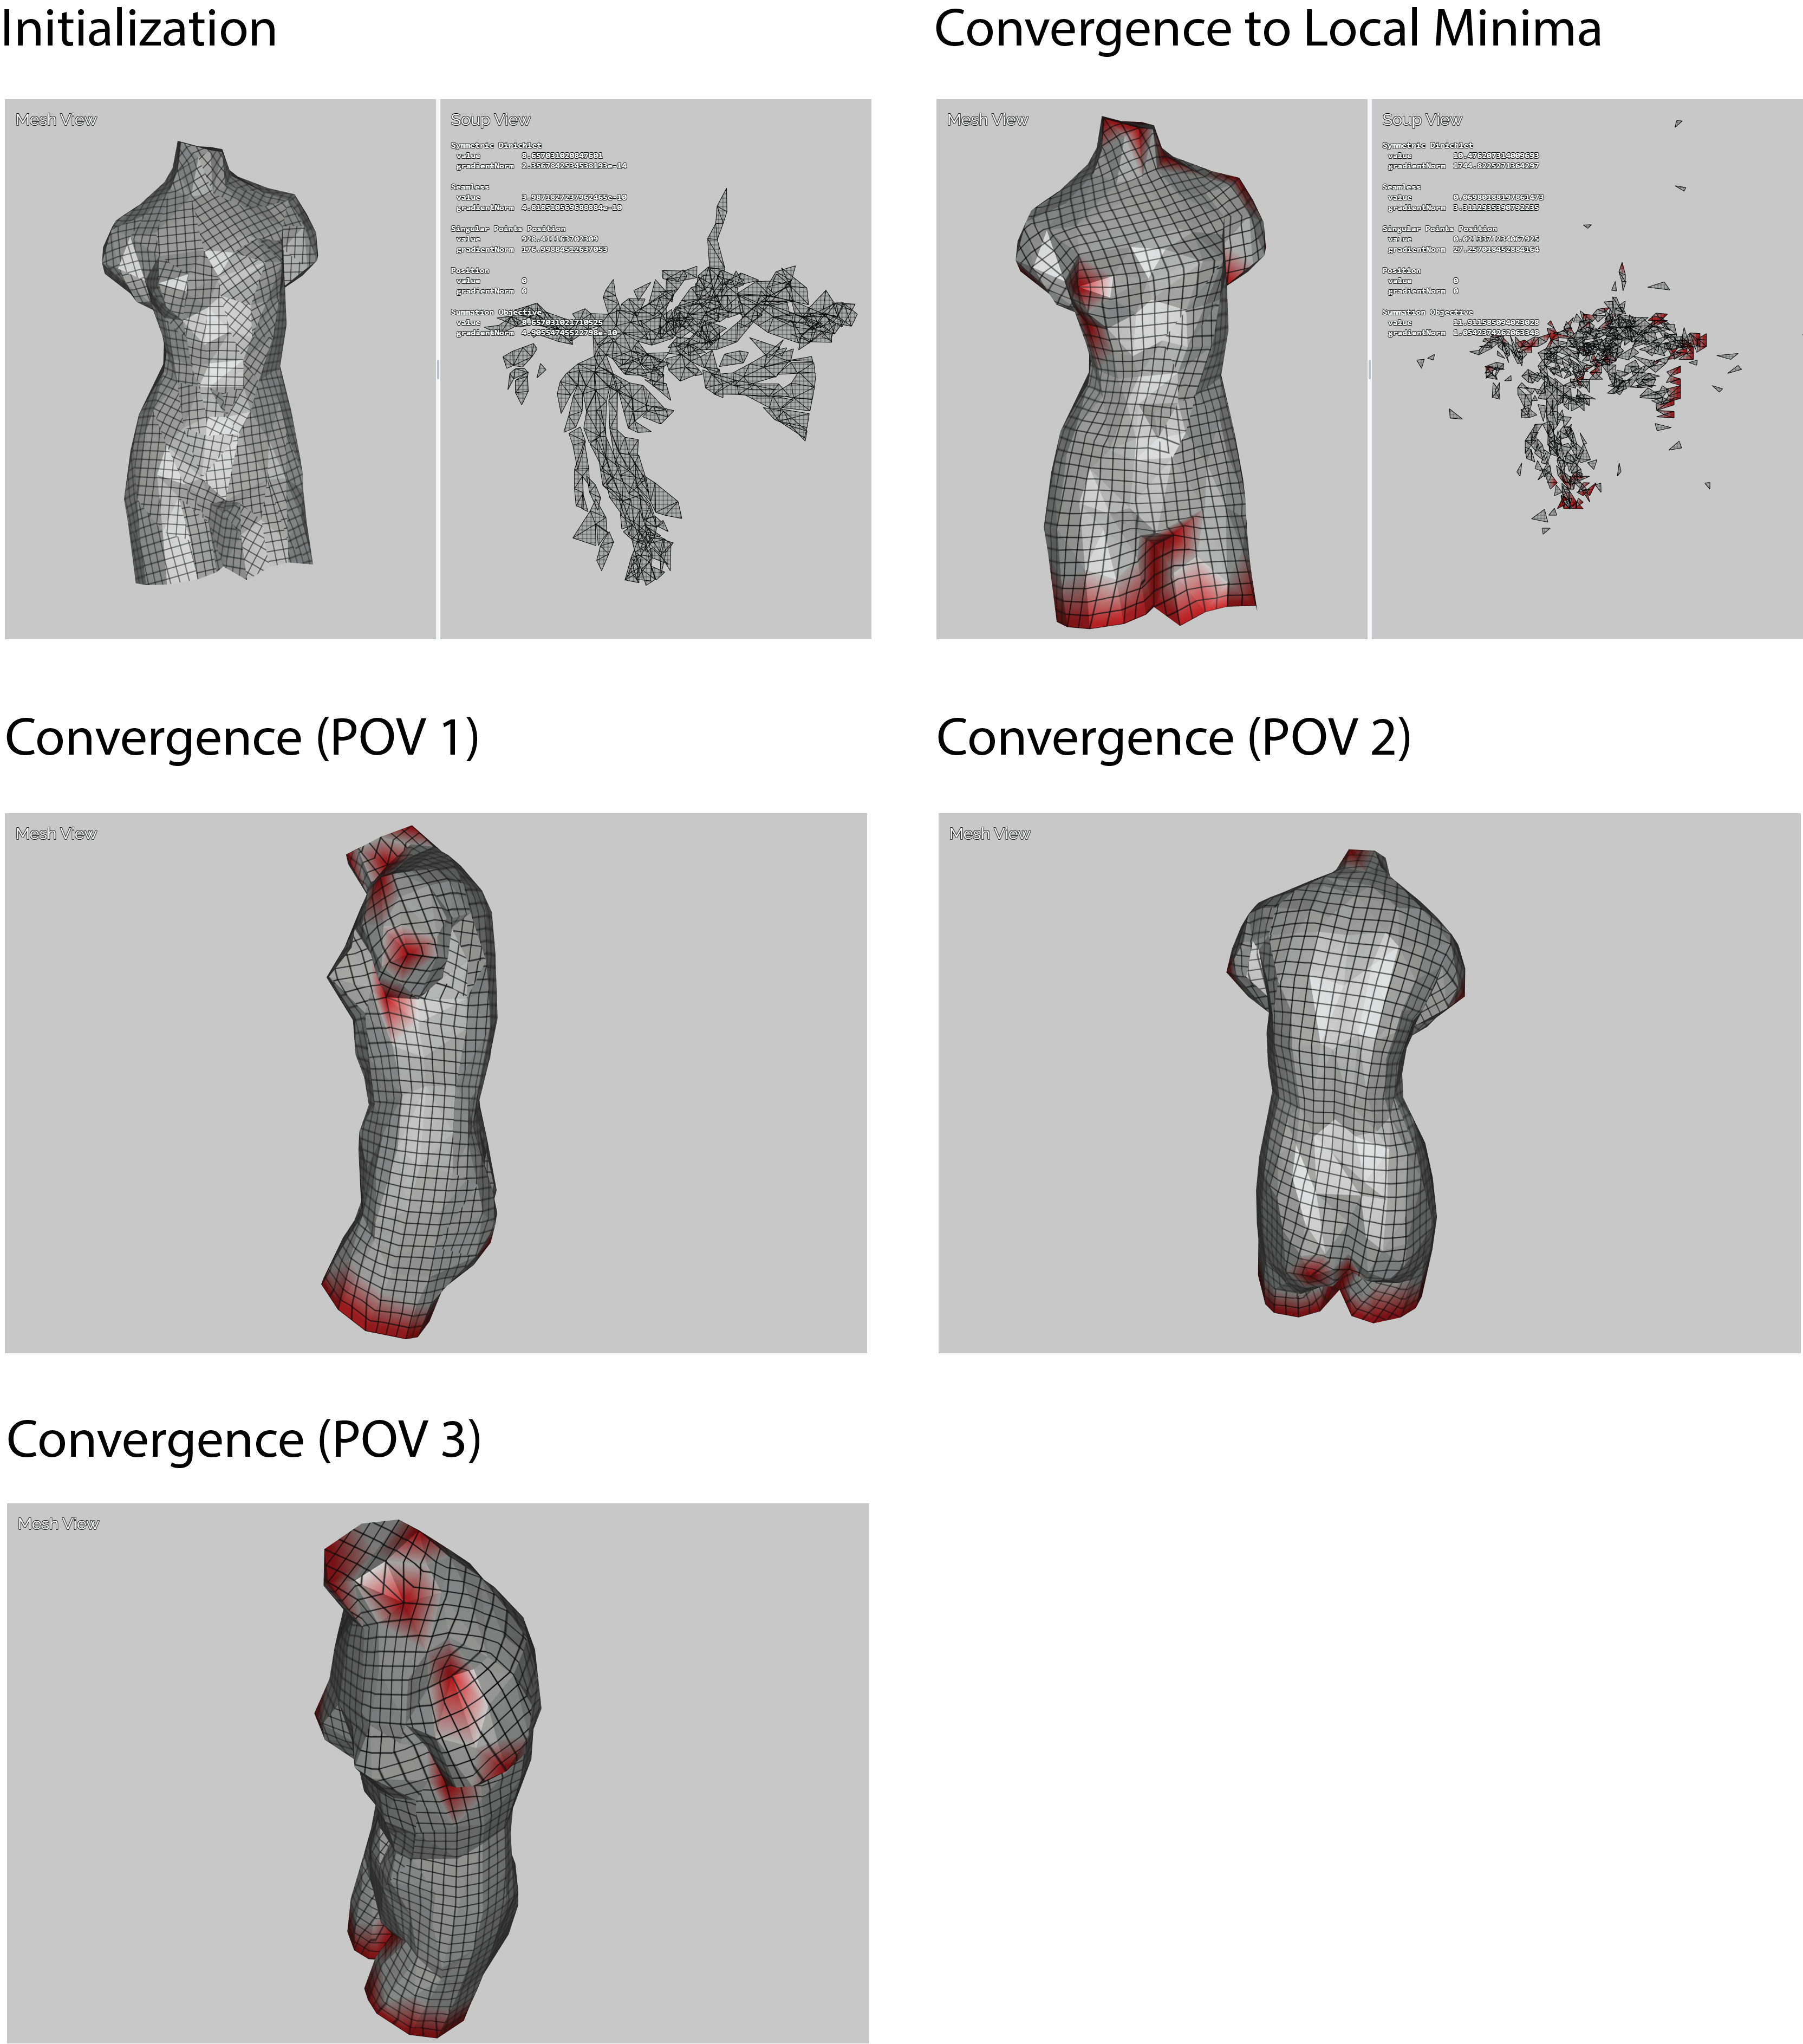
\includegraphics[width=14cm]{figures/results/venus.png}
\caption[Venus Model]{}
\end{figure}
\newpage
\section{Retinal Model}
\begin{figure}[ht]
\centering
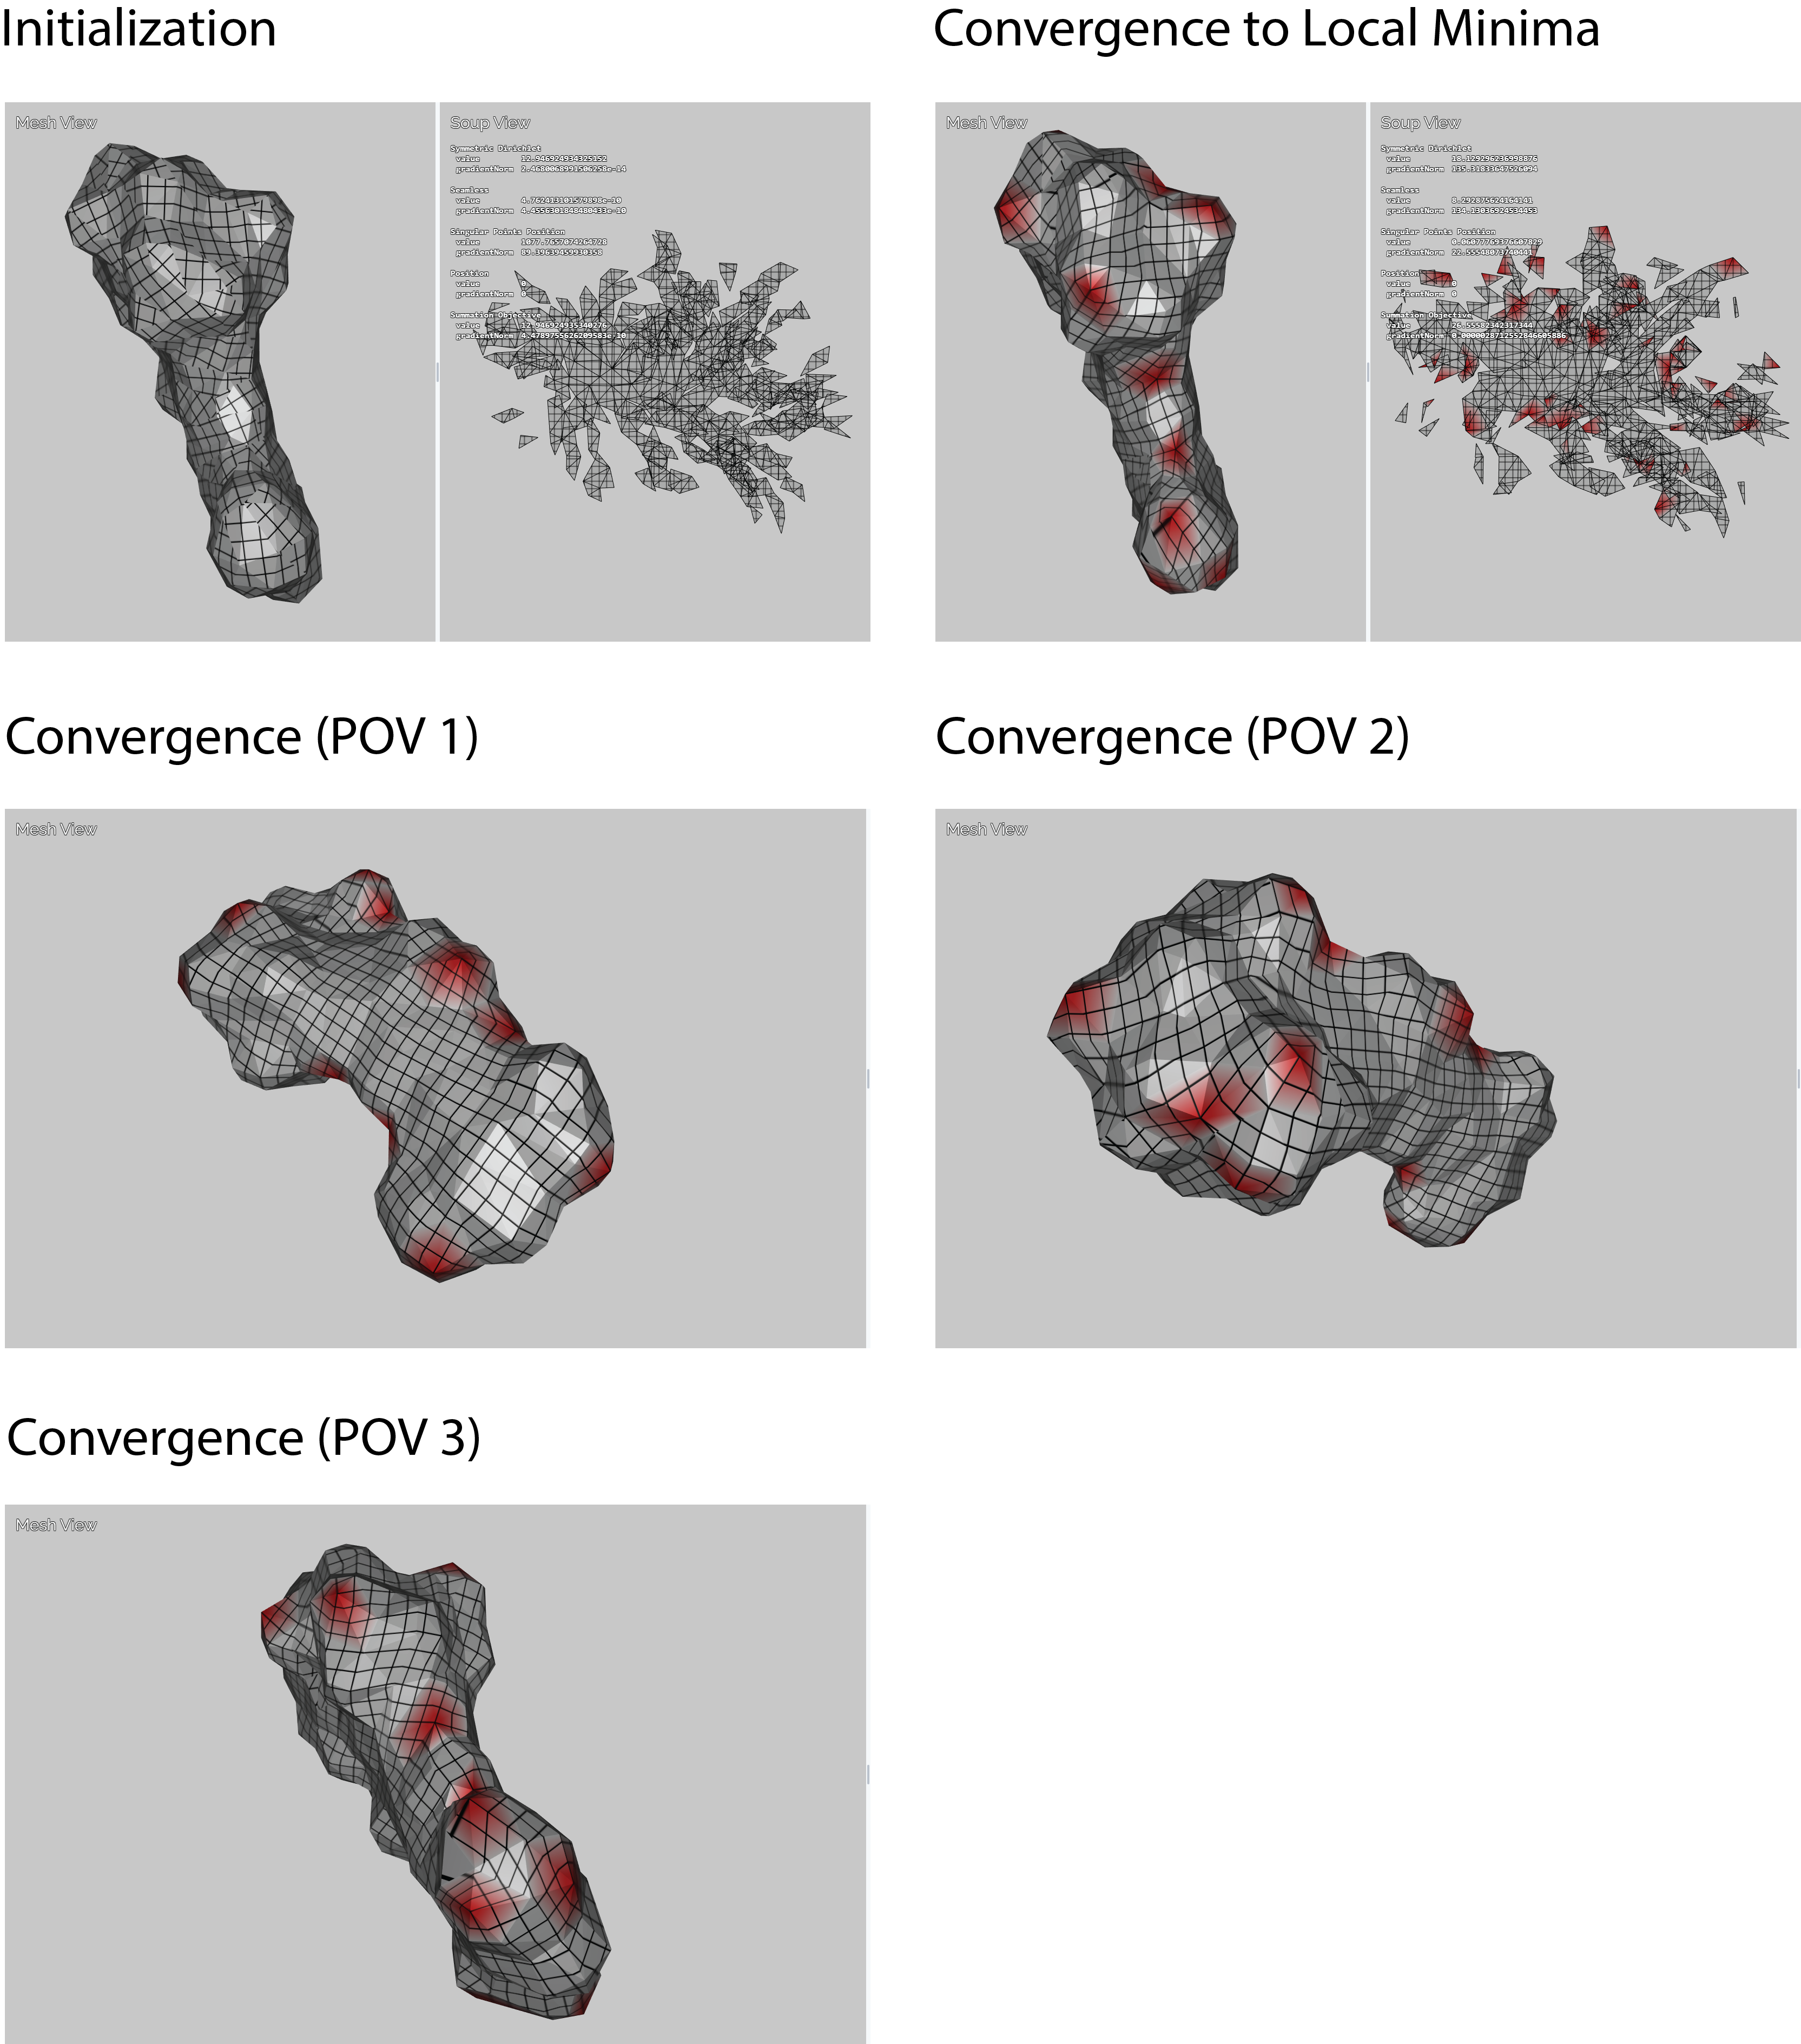
\includegraphics[width=14cm]{figures/results/retinal.png}
\caption[Retinal Model]{}
\end{figure}